
\subsection{Distributed stream processing}

In order to solve real life tasks with high-velocity data, the stream processing systems can be used as a solution. The main idea of these systems is as follows. Every piece of data is enters and exists the system one by one. After entering, every element then evenly distributed using sharding technique for balancing the workload. This allows to produce a low latency and provide scalablity. The examples of such systems are Apache Flink [?], Google's MillWheel [?], Spark Streaming[?] or Apache Storm[?].

In this work, our computations based on FlameStream \cite{kuralenok2018flamestream} distributed model, which provides the following advantages:

\textbf{Determinism.} The result of computing is determined only by input data and remain the same between independent launches. This makes whole classifying process more predictable as it was discussed in \cite{stonebraker20058} Rule 4. In addition, the concept ensures an opportunity for tests that validate the whole pipeline. FlameStream determinism is considered as lightweight.

\textbf{Exactly-once.} Unlike the others stream processing systems, FlameStream produces results with lower latency using the same data processing. FlameStream process data in exactly-once manner, which ensures a low latency with almost no overhead.

These advantages allows us to create a classifier with better performance and due to the determinism and exactly-once delivery guarantee ensure consistent results.

\subsection{Data flow}

\subsubsection{Computational pipeline}

Similar to other stream processing systems, FlameStream is doing its calculations using a computational graph. This graph is  commonly referred to as logical graph. Logical graph transforms into actutal physical for processing computations. The graph provides a scheme of data flow and can be presented like this:

\begin{figure}[htbp]
  \centering
  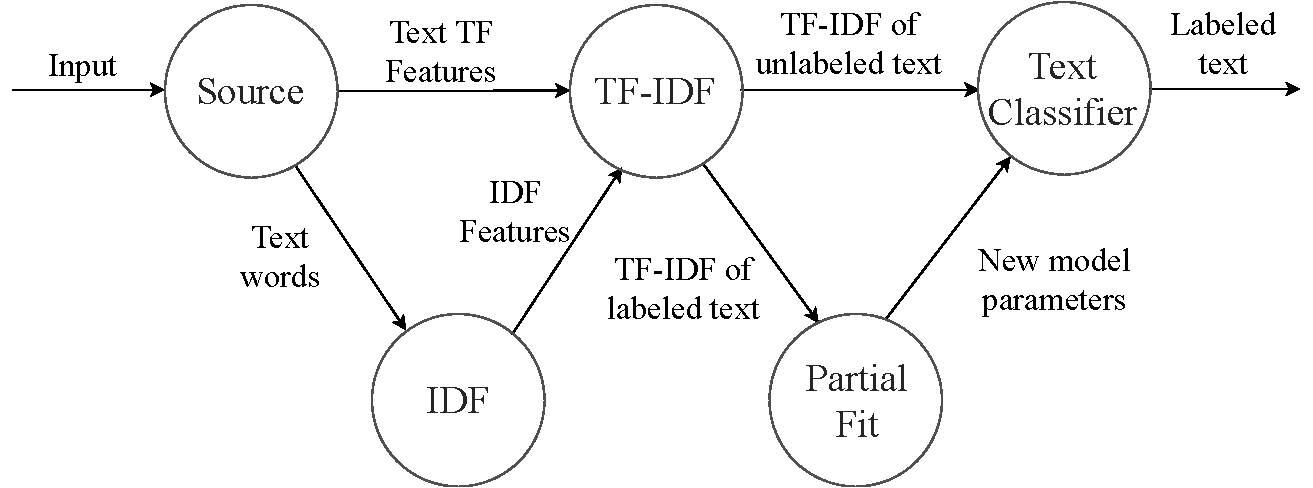
\includegraphics[scale=0.48]{pics/logical-graph}
  \caption{The logical pipeline}
  \label {logical graph}
\end{figure}

The Figure 1 illustrates the principle pipeline. An oriented edge indicates the flow and kind of the data. Every vertex in the graph represents a processing unit such as a single computer or a cluster. The initial text document splits into two computations: the first is calculates term frequencies and the second calculates inverse document frequencies. TF features is computed on the same machine, where the document is arrived, and passes further into TF-IDF vertex. On the other hand, IDF features computations is balanced among all shards. The process of balancing the workload is same as in FlameStream. The range $[0, 2^{32} - 1]$ is divided into equal parts by the number of the shards. Every single shard is responsible for its own range. Hash of each word defines what shard will be used for further IDF computation. In case of words with high frequency such as conjunctions or prepositions, we add to them the salt to the end thereby distributing all the words between the shards evenly. Results from IDF vertex in TF-IDF vertex aggregate with TF features and text classifier receives TF-IDF features of the document. The classifier outputs labelled document and this document returns to the user.

\subsubsection{Dealing with concept drift}

Concept drift is a phenomenon of changing users' interests from time to time, which usually depends on recent events, and results in shifting the distribution of text classes to particular ones. Essentially, this may affect correctness of the pipeline, more specifically, the computing of the IDF features. To overcome the issue, we use windowed IDF calculation: concrete IDF values will be provided based on input within the window. For instance, the window can be set to a day or a week. This scheme allows to deal with the sudden changes of the topics.

\subsubsection{Partial fit}

\begin{figure}[htbp]
  \centering
  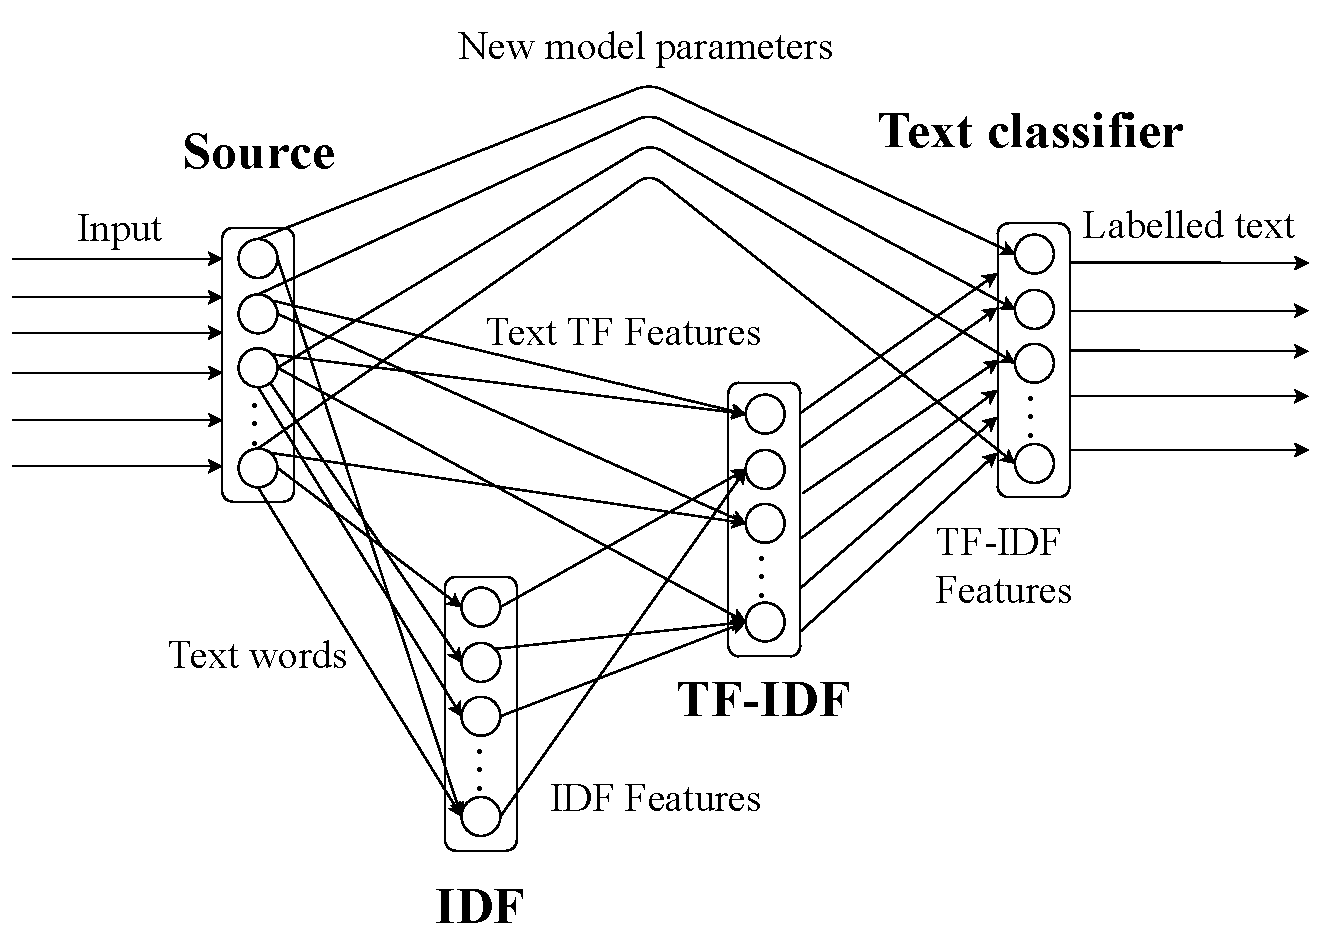
\includegraphics[scale=0.38]{pics/physical-graph}
  \caption{The physical pipeline}
  \label {physical graph}
\end{figure}

The Figure 2 shows the physical graph of the pipeline for real calculations. Input text can be received by any machine. After that, during IDF computing the corresponding inputs reshuffle for balancing workload and final TF-IDF features aggregate in TF-IDF stage. In final stage text classifier obtains a label for the text and returns to the user.

In addition, the two figures above provide a scheme for a partial fitting. Some of the text documents is labelled and such documents accumulate in the Partial Fit vertex. Additional training is triggered by a special element, which is submitted similarly to the input. This process is analogous to punctuation processing \cite{tucker2003exploiting}. The conditions, when the partial fitting starts, can be chosen arbitrarily, for example, train on each 10000 documents. During this process, the existing classifier's weights are being updated as it is described below. After that, new weights is distributed among the system and the classification continues. 

\subsection{ML model}

The classifier's model can be chosen independently from other computations. In our case, we use Multinomial Logistic Regression. The initial classifier weights provided by a pretrain process. 

Fitting process can be described as follows. Cost function is illustrated below:

\begin{center}

$$ J(W) = -\frac{1}{m} \sum \limits_{i = 1}^{m} \sum \limits_{j = 1}^{k} \mathbbm{1}_{\{y^{(i)} == j\}} \cdot \log \frac{\exp\left({W_{j}^Tx^{(i)}}\right) }{\sum \limits_{l = 1}^{k}  \exp\left({W_{l}^Tx^{(i)}}\right) }$$ 
 $$ + \; \lambda_1 ||W||_1 + \lambda_2 ||W - W_{prev}||_2 $$

\end{center} 

The number of points in new dataset is denoted as $m$. The number of classes is $k$. New weights are designated as $W$ and previous weights are $W_{prev}$.

The gradient of the cost function can be put as:

$$ \nabla_{W_j} \; J(W) = -\frac{1}{m} \sum \limits_{i = 1}^{m} \left[ x^{(i)} \left( \mathbbm{1}_{\{y^{(i)} == j\} } - \frac{\exp\left({W_{j}^Tx^{(i)}}\right)}{\sum \limits_{l = 1}^{k}  \exp\left({W_{l}^Tx^{(i)}}\right)} \right) \right] $$

We calculate the gradient of each component and update the weights in one iteraton of the gradient descent. Maximum number of iterations of the descent is 100.